\newpage
\hypertarget{M2TSettingUp vis}{}
\subsection{Initializing the project}
\visHeader

\begin{enumerate}

\item[$\blacktriangleright$] Your EA unexpanded project browser should now resemble Fig.~\ref{ea:mocaTagged}. You can see that your project is already populated
with the metamodel for our generic tree. To differentiate this from other trees (ANTLR parse tree and abstract syntax tree, XML DOM tree, \ldots) we refer to it
as \texttt{MocaTree}.

\begin{figure}[htpb]
\begin{center}
  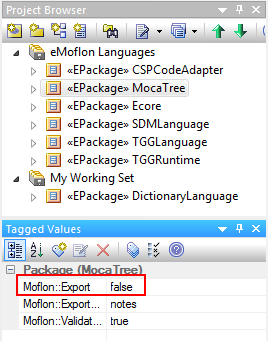
\includegraphics[width=0.4\textwidth]{ea_mocaTaggedValues}
  \caption{figureCaption}
  \label{ea:mocaTagged}
\end{center}
\end{figure}

\item[$\blacktriangleright$] Note that the \texttt{MocaTree} package has a special tagged value \texttt{Moflon::Export} set to \texttt{false}\footnote{The
``Tagged Values'' window can be opened by going to ``View/Tagged Values''}. This ensures that the package is \emph{ignored} when exporting. As with all standard
metamodels (e.g., Ecore or the SDM metamodel) the \texttt{MocaTree} package in EA should be regarded as read-only and is only required in the EA project so that
SDMs can refer to the classes defined in the package. The corresponding Java code is provided by our Eclipse plugin and is added automatically to the Java build
path whenever necessary.

\item[$\blacktriangleright$] Go ahead and inspect the \texttt{MocaTree} metamodel (Fig.~\ref{ea:mocaTree}). It basically combines concepts from a filesystem
(folders and files), XML concepts (text-only nodes and attributes), and a general indexed\footnote{The index attribute in \texttt{TreeElement} can be used to
demand a certain \emph{order} of nodes in an SDM, which is otherwise not guaranteed by default (order is in general non-deterministic).} containment hierarchy.

\begin{figure}[htpb]
\begin{center}
  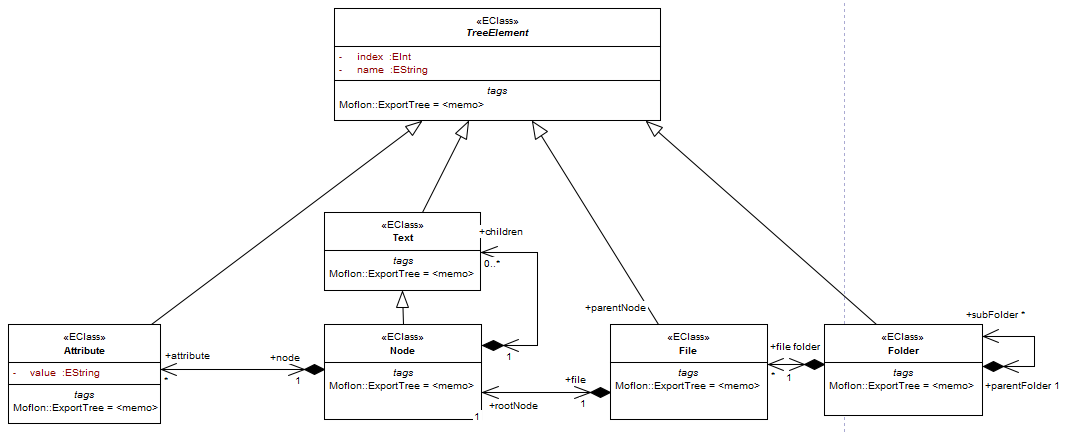
\includegraphics[width=\textwidth]{ea_metamodelMocaTree}
  \caption{figureCaption}
  \label{ea:mocaTree}
\end{center}
\end{figure}
 
\newpage

\item[$\blacktriangleright$] Add a package to your \texttt{My Working Set} node named \texttt{DictionaryCodeAdapter}. Then add a new TGG diagram
(Fig\texttt{blahhh}) with the same name -- Make sure you set the \emph{input} source and target correct. We have mentioned in previous sections that those
titles generally don't imply direction, when building one direction first, where it starts matter. (Explain)

\item[$\blacktriangleright$]with a single correspondence type between \texttt{textt} and \texttt{textt2} so that your workspace resembles Fig.\texttt{blahhh}
Then add an

\begin{figure}[htpb]
\begin{center}
  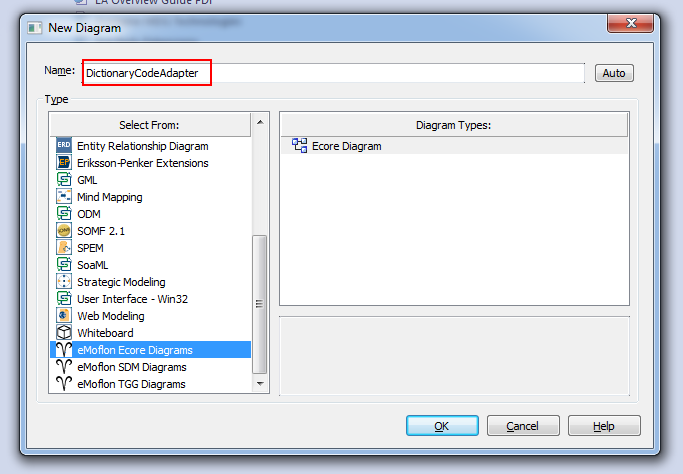
\includegraphics[width=0.8\textwidth]{ea_transformerDiagram}
  \caption{figureCaption}
  \label{ea:newTransformer}
\end{center}
\end{figure}

Our conventions and workflow state that this \emph{code adapter} is a package that contains the tree-to-model transformation logic. This could be integrated
directly in the corresponding metamodel (\texttt{Dic\-tion\-ary\-Language}), but here a separation makes sense as there could be \emph{different} code adapters
for the \emph{same} language.

\item[$\blacktriangleright$] Save and validate your updated project from EA.\footnote{Refer to Part II, Section 2.8 if unsure} You can ignore the
\texttt{EmptyPackageNotAllowed} error for now -- we'll complete the \texttt{Transformer} diagram in a moment. Our goal right now is to generate
\texttt{DictionaryCodeAdapter}, so return to and refresh your Eclipse workspace. 

\jumpSingle{subSec:setupParser}

\end{enumerate}
